\documentclass[11pt,a4paper]{article}

\usepackage[utf8]{inputenc}
\usepackage[T1]{fontenc}
\usepackage[a4paper,margin=1in]{geometry}
\usepackage{amsmath,amssymb,amsfonts}
\usepackage{booktabs,array,longtable}
\usepackage{graphicx}
\usepackage{xcolor}
\usepackage{listings}
\usepackage[inline]{enumitem}
\usepackage{hyperref}
\usepackage{setspace}
\usepackage{fancyhdr}
\usepackage{titlesec}



\setstretch{1.08}
\setlength{\parindent}{0pt}
\setlength{\parskip}{0.6em}

\pagestyle{fancy}
\fancyhf{}
\setlength{\headheight}{14pt}
\lhead{Assignment 5}
\rhead{Layout Optimization for LCoE}
\cfoot{\thepage}

\titleformat{\section}{\large\bfseries}{\thesection.}{0.5em}{}
\titleformat{\subsection}{\normalsize\bfseries}{\thesubsection}{0.5em}{}

\definecolor{codegray}{RGB}{248,248,248}
\definecolor{codeborder}{RGB}{220,220,220}

\lstdefinestyle{mystyle}{
	backgroundcolor=\color{codegray},
	frame=single,
	rulecolor=\color{codeborder},
	basicstyle=\ttfamily\small,
	breaklines=true,
	columns=fullflexible,
	keepspaces=true,
	showstringspaces=false,
	tabsize=4
}
\lstset{style=mystyle}

\title{\textbf{Assignment 5}\\
	\normalsize Layout Optimization for LCoE}
\author{Chinmay S Patil}
\date{}

\graphicspath{{./}}

\begin{document}
	\maketitle

	%% ─────────────────────────────────────────────────────────────────────────────
	\section{Task 1: Wind Rose at Hub Height}
	%% ─────────────────────────────────────────────────────────────────────────────

	Wind speed and direction data were downloaded from the New European Wind Atlas (NEWA)
	for Marienplatz, Munich, covering the full mesoscale time series from 1989 to 2022.
	The raw data were provided at 10\,m height and scaled to hub height (120\,m) using
	the power-law wind shear model with exponent $\alpha = 0.20$:
	\[
		U(h) = U_{\text{ref}}\left(\frac{h}{h_{\text{ref}}}\right)^{\alpha}
	\]

	\begin{figure}[h!]
		\centering
		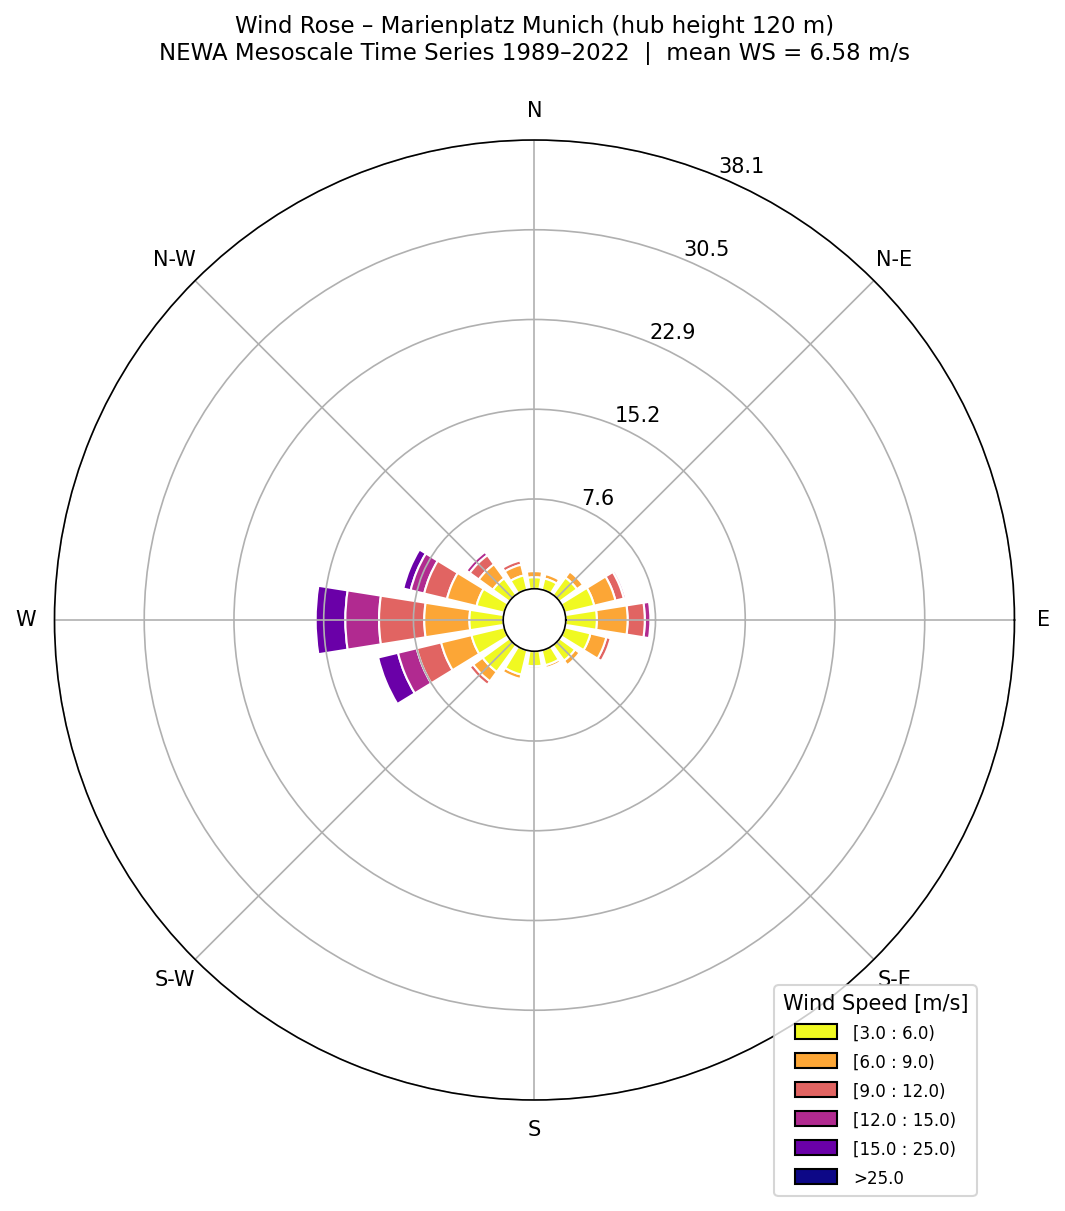
\includegraphics[width=0.65\linewidth]{task1_windrose.png}
		\caption{Wind rose at Marienplatz, Munich -- NEWA Mesoscale Time Series 1989--2022
			(hub height 120\,m, mean wind speed = 6.58\,m/s).}
		\label{fig:windrose}
	\end{figure}

	The wind rose shows a strongly dominant westerly and south-westerly wind regime.
	Wind speeds of 6--9\,m/s (orange) and 9--12\,m/s (salmon) are most frequent, and
	higher speeds above 15\,m/s (purple) also arrive predominantly from the west.
	Wind activity from the north and south is negligible.
	The mean wind speed at hub height is \textbf{6.58\,m/s}.

	This strongly directional resource is a critical input for the layout optimisation
	in Task~3: turbines aligned in the west--east direction will experience the largest
	wake losses under the prevailing wind.

	%% ─────────────────────────────────────────────────────────────────────────────
	\section{Task 2: Baseline Wind Farm Evaluation}
	%% ─────────────────────────────────────────────────────────────────────────────

	\subsection{Setup}

	The initial layout places eight IEA 3.4\,MW turbines in a $4\times 2$ grid
	centred within the 2.8\,km\,$\times$\,2.8\,km boundary, with the substation at
	the centre point.  Wake interactions were evaluated with the Gauss wake model
	(default parameters) in FLORIS, using a wind shear exponent of $\alpha = 0.20$
	and turbulence intensity TI\,$= 6\,\%$.

	\subsection{Results}

	\begin{lstlisting}
	AEP:                     68.36  GWh/yr
	Capacity Factor:         28.95  %
	Farm Efficiency:         77.62  %
	LCoE:                    62.40  $/MWh
	Profitability Index:      0.119  --
	\end{lstlisting}

	Because the turbines are aligned east--west and the dominant winds arrive from
	the west, the rear row suffers substantial wake losses, reducing AEP and farm
	efficiency.  The baseline LCoE of 62.40\,\$/MWh is below the electricity price
	of 67\,\$/MWh, so the project is marginally profitable, but there is clear room
	for improvement through layout optimisation.

	%% ─────────────────────────────────────────────────────────────────────────────
	\section{Task 3: COBYLA Layout Optimisation}
	%% ─────────────────────────────────────────────────────────────────────────────

	\subsection{Method}

	\texttt{scipy.optimize.minimize} with the \textbf{COBYLA} (Constrained
	Optimization BY Linear Approximation) gradient-free method was used to optimise
	the 16 turbine coordinates ($8\times x$,\;$8\times y$) so as to minimise the
	LCoE of the wind farm.  The following constraints were enforced:

	\begin{itemize}[leftmargin=1.5em]
		\item All turbines must remain within the 2.8\,km\,$\times$\,2.8\,km boundary.
		\item Minimum turbine-to-turbine separation of $2D = 260$\,m for all pairs.
	\end{itemize}

	\subsection{Convergence}

	\begin{figure}[h!]
		\centering
		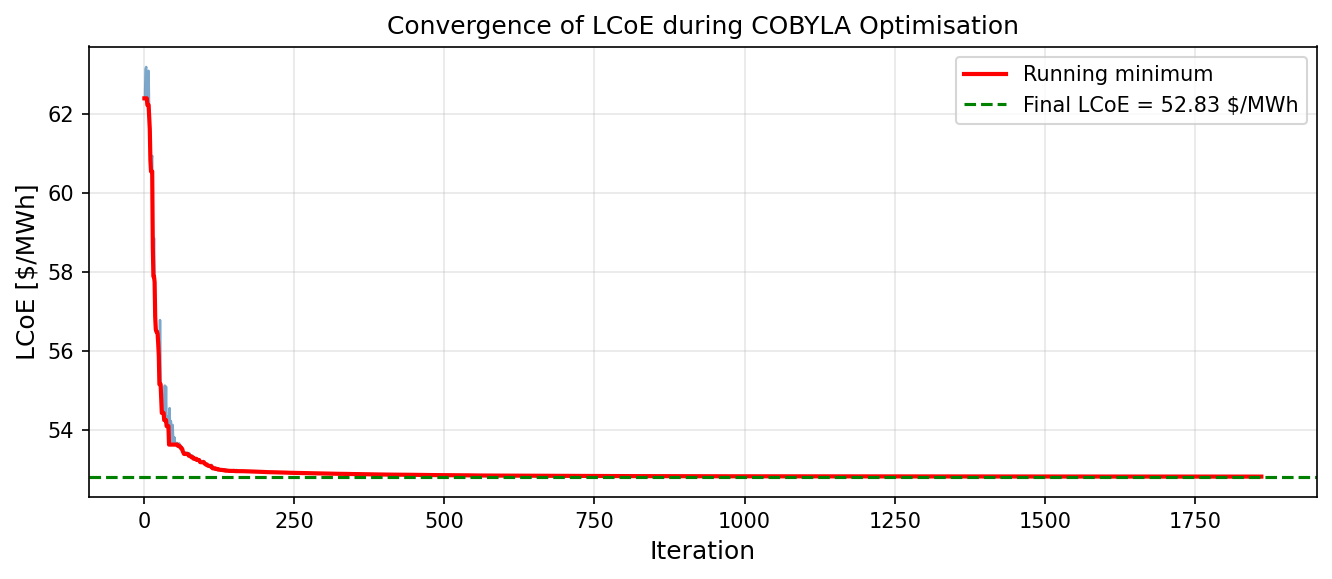
\includegraphics[width=\linewidth]{task3_convergence.png}
		\caption{Convergence of LCoE during COBYLA optimisation.  The running minimum
			(red) drops rapidly within the first $\sim$250 iterations and flattens at
			the final optimum of 52.83\,\$/MWh (green dashed line).}
		\label{fig:convergence}
	\end{figure}

	The optimiser starts at approximately 63\,\$/MWh and converges rapidly; the
	objective is essentially flat after iteration $\sim$500, confirming that a local
	optimum has been reached.  The total number of function evaluations was 1\,900.

	\newpage

	\subsection{Optimised Layout}

	\begin{figure}[h!]
		\centering
		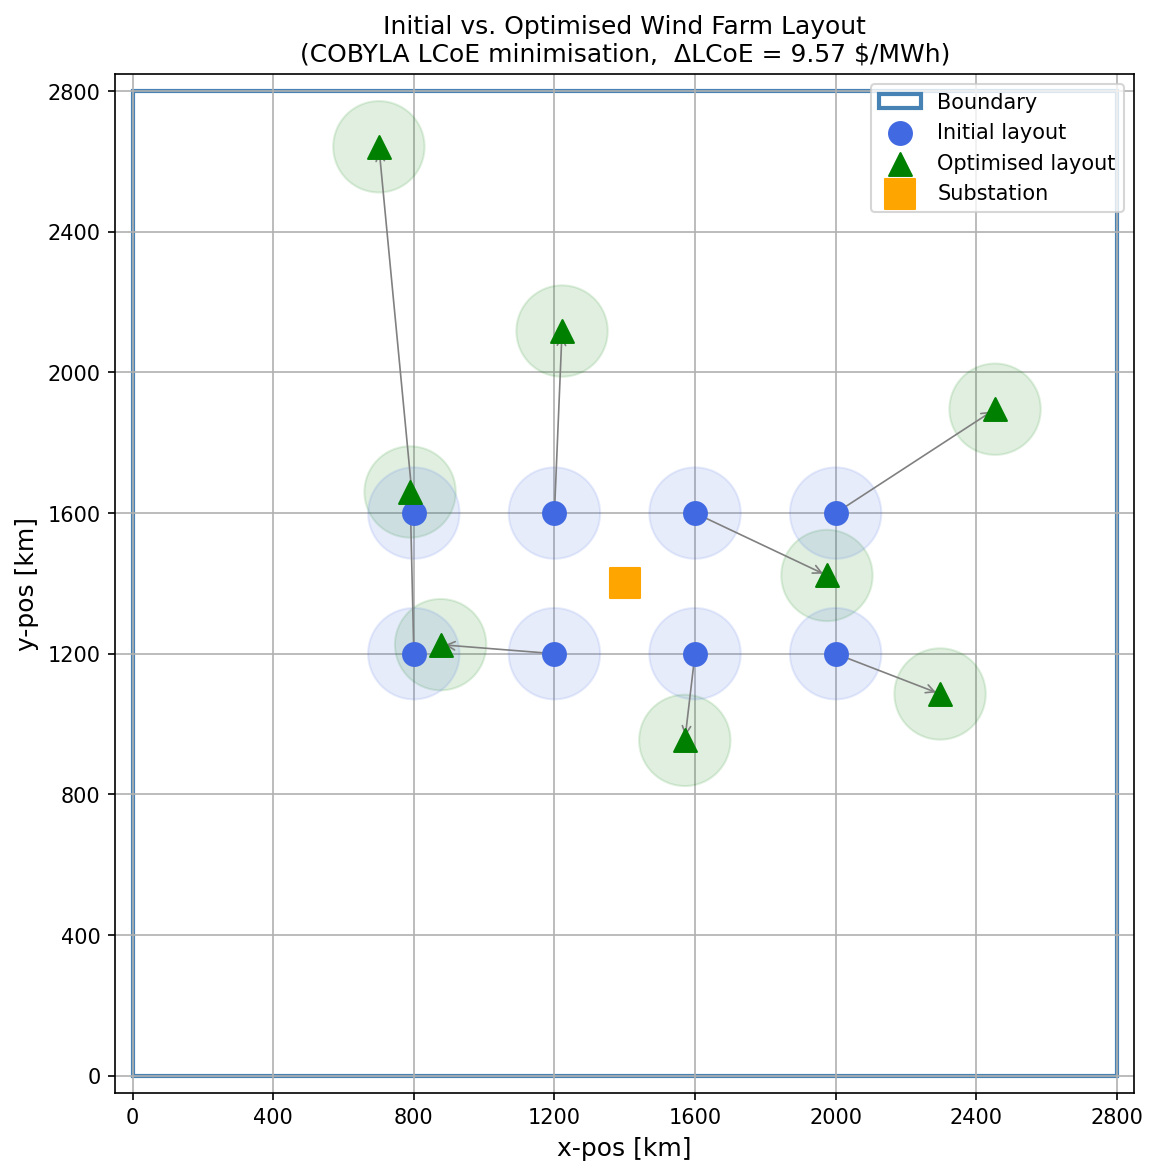
\includegraphics[width=0.78\linewidth]{task3_layout.png}
		\caption{Initial (blue circles) vs.\ optimised (green triangles) wind farm
			layout.  Arrows indicate turbine displacement.
			$\Delta\mathrm{LCoE} = 9.57$\,\$/MWh.}
		\label{fig:layout}
	\end{figure}

	The optimised layout shows several key changes relative to the baseline:
	\begin{itemize}[leftmargin=1.5em]
		\item Turbines aligned west--east in the baseline have been spread in the
		      north--south direction, reducing wake overlap under the dominant westerly wind.
		\item Several turbines moved towards the boundary edges to maximise mutual
		      separation.
		\item All minimum spacing constraints ($2D = 260$\,m) are satisfied, as
		      confirmed by the non-overlapping exclusion circles.
	\end{itemize}

	\subsection{Comparison of Results}

	\begin{center}
		\begin{tabular}{lrrl}
			\toprule
			\textbf{Parameter} & \textbf{Initial} & \textbf{Optimised} & \textbf{Unit} \\
			\midrule
			AEP                   & 68.36 & 87.28 & GWh/yr \\
			Capacity Factor       & 28.95 & 36.96 & \%     \\
			Farm Efficiency       & 77.62 & 99.11 & \%     \\
			LCoE                  & 62.40 & 52.83 & \$/MWh \\
			$\Delta$LCoE          & \multicolumn{2}{c}{9.57} & \$/MWh \\
			Profitability Index   &  0.119 &  0.462 & --    \\
			\bottomrule
		\end{tabular}
	\end{center}

	\subsection{Profitability Discussion}

	The optimised LCoE of \textbf{52.83\,\$/MWh} is well below the electricity price
	of 67\,\$/MWh, confirming that the project has become clearly profitable after
	optimisation.  The $\Delta\mathrm{LCoE}$ of 9.57\,\$/MWh was achieved purely by
	repositioning turbines, with no additional capital expenditure.

	The farm efficiency improvement from 77.62\,\% to 99.11\,\% demonstrates that
	wake losses were substantially reduced, driving up AEP and reducing LCoE.  This
	underlines layout optimisation as a highly cost-effective measure -- a finding
	consistent with the strongly directional wind resource observed at the Munich site.

\end{document}